\section{Evaluation}
\label{sec:evaluation}

In this section, we quantify the benefits of using a wireless mesh in crowd-shared home networks for public Internet access. In Section \ref{evaluation:environment}, we present the simulation environment, the modeling of router on/off periods, and the metrics used to evaluate the efficiency of the wireless mesh. Section \ref{evaluation:results} provides a comparative study of crowd-shared home networks with and without a wireless mesh based on our simulation results.

\subsection{Simulation Environment}
\label{evaluation:environment}


\begin{figure}[h]
\begin{center}
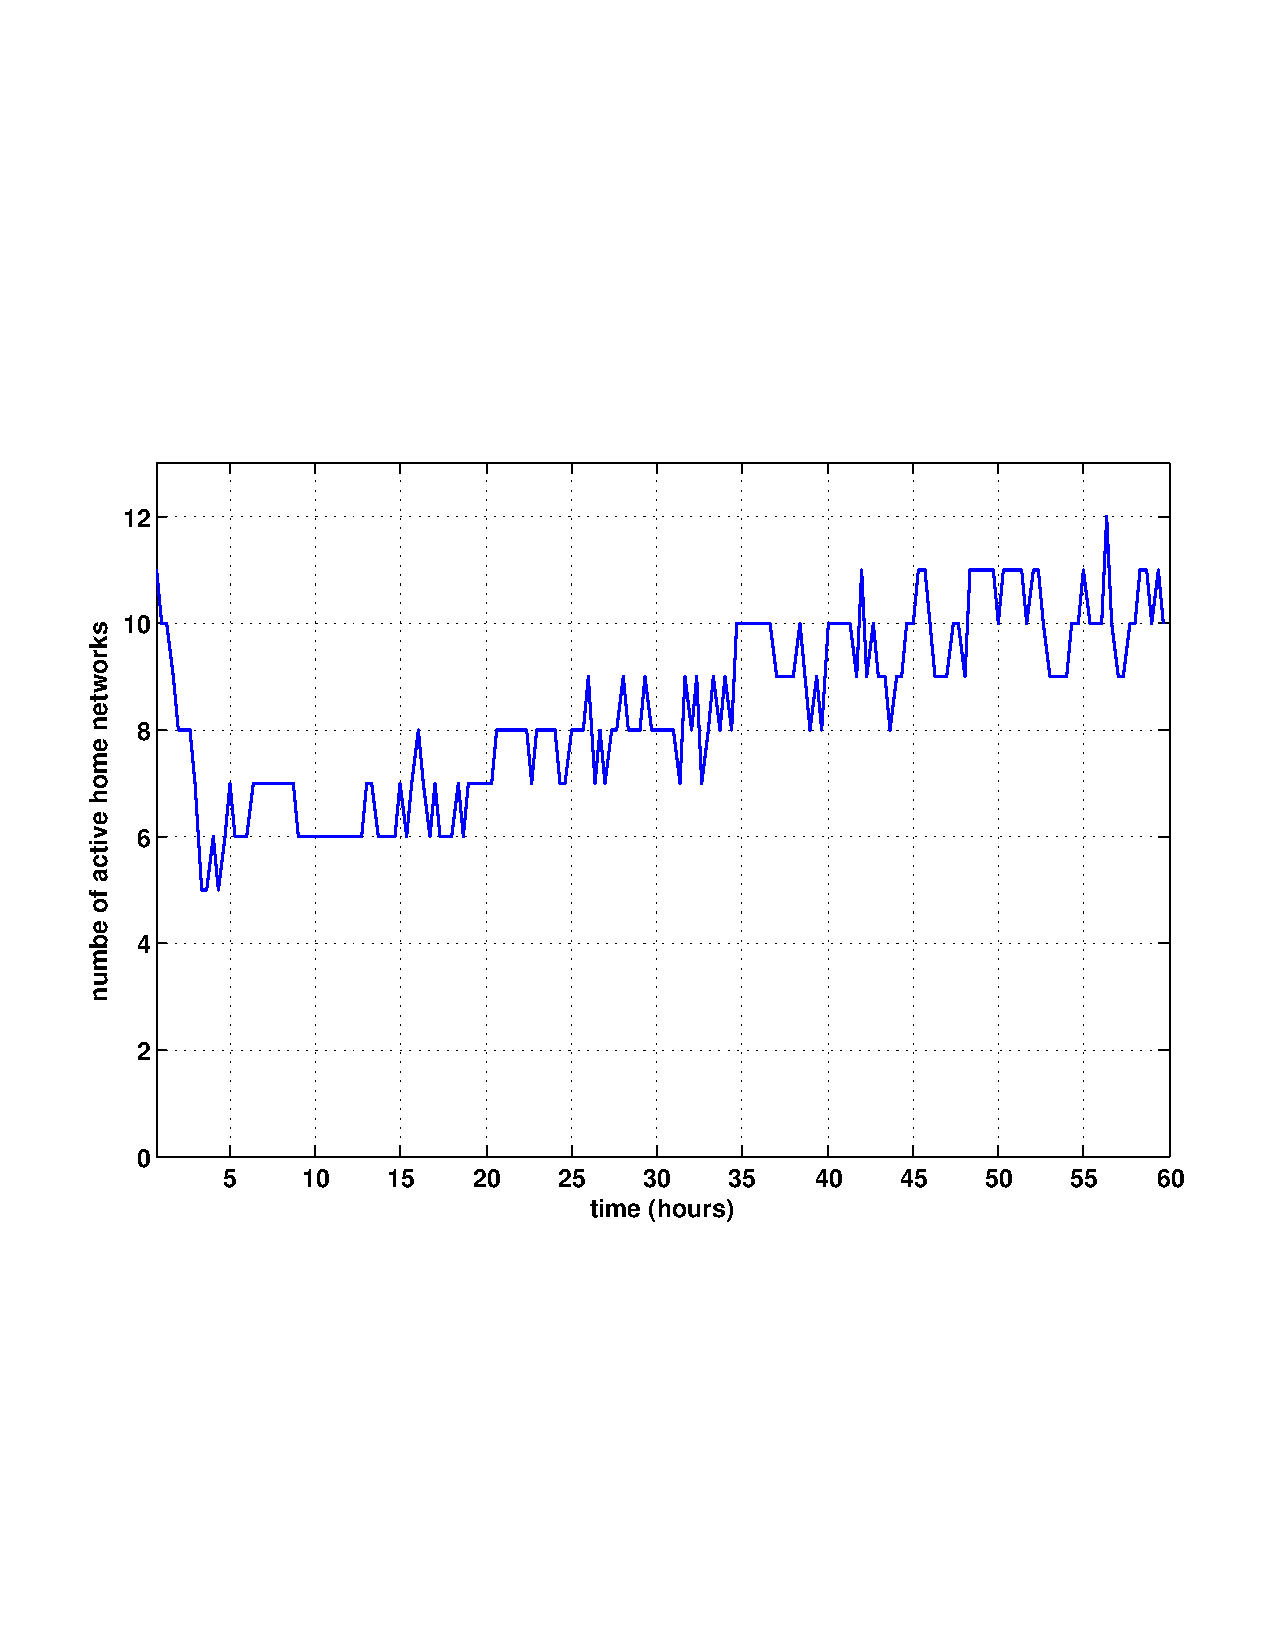
\includegraphics[width=1\linewidth]{../../results/simulation/on_routers2.pdf}  
\caption{Number of active home routers.}
\label{fig:active_routers}
\end{center}
\end{figure}


\subsection{Simulation Results}
\label{evaluation:results}

Initially, we measure the shared bandwidth utilization and request acceptance rate with an arrival rate of 50 flows per minute over a 60-hour period. Fig. \ref{fig:utilization} illustrates a low utilization of the shared bandwidth without a wireles mesh during the whole period, although there is high demand for Internet access by guest users attached to the various home networks. In contrast, a wireless mesh allows to capitilize the unused capacity and accommodate a larger volume of guest user traffic. More precisely, according to Fig. \ref{fig:utilization} guest user traffic redirection through the wireless mesh results in the full utilization of the bandwidth shared by home network users. Furthermore, crowd-shared home networks with a wireless mesh can accommodate substantially higher guest user traffic, as depicted in Fig. \ref{fig:acceptance}. This stems from the high utilization of the shared bandwidth. 

\begin{figure}[h]
\begin{center}
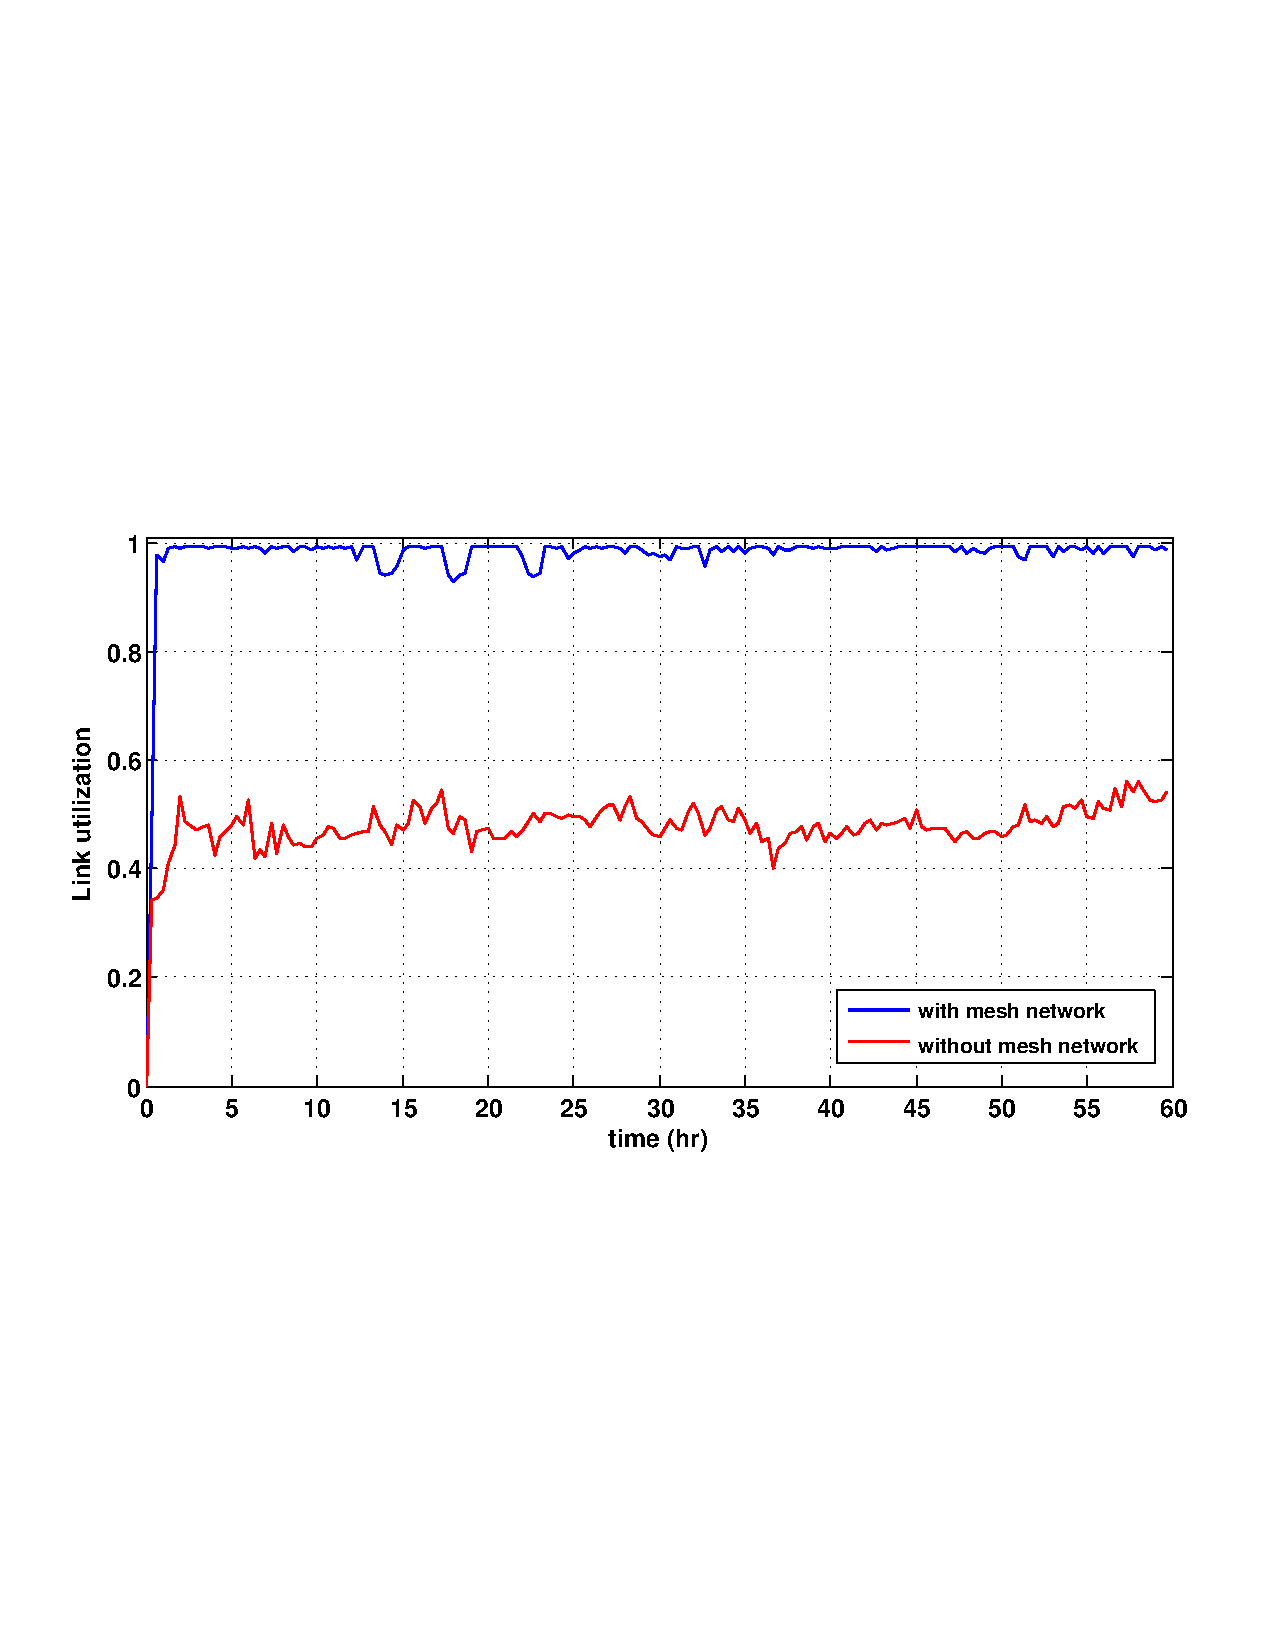
\includegraphics[width=1\linewidth]{../../results/simulation/utilization.pdf}  
\caption{Shared bandwidth utilization.}
\label{fig:utilization}
\end{center}
\end{figure}

\begin{figure}[h]
\begin{center}
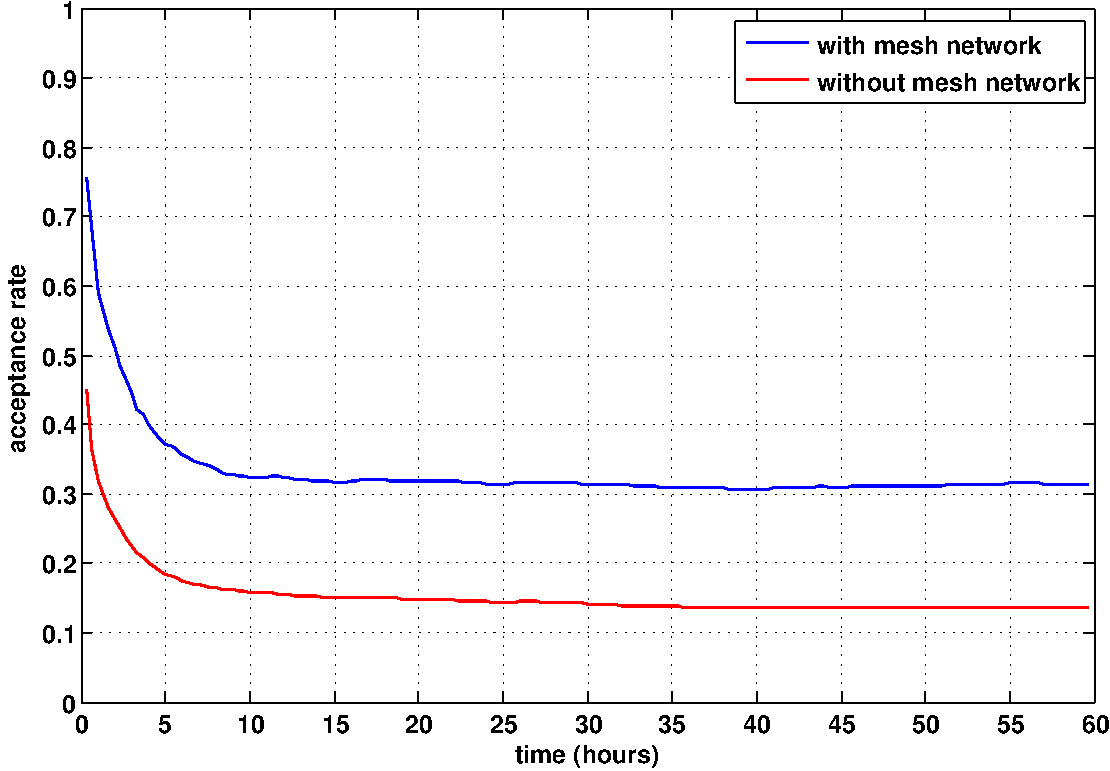
\includegraphics[width=1\linewidth]{../../results/simulation/acceptance_rate.pdf}  
\caption{Guest user traffic acceptance rate.}
\label{fig:acceptance}
\end{center}
\end{figure}

We further measure the shared bandwidth utilization with a wide range of guest user traffic demands. In this respect, Fig. \ref{fig:acceptance} illustrates the shared bandwidth utilization with diverse flow arrival rates, ranging from 10 to 100 flows per minute. This simulation result corroborates the efficiency of the wireless mesh for various traffic loads, as the shared bandwidth utilization always remains very high. Without the presence of a wireless mesh, Fig. \ref{fig:acceptance} shows poor bandwidth utilization, especially with low guest user traffic demand. In this particular case, the inability to redirect guest user traffic to home networks with available bandwidth results in wasting most of the shared bandwidth. Eventually, our simulation results show the significant benefit that a wireless mesh can bring in crowd-shared home networks, by effectively pooling shared resources across the interconnected home networks. 

\begin{figure}[h]
\begin{center}
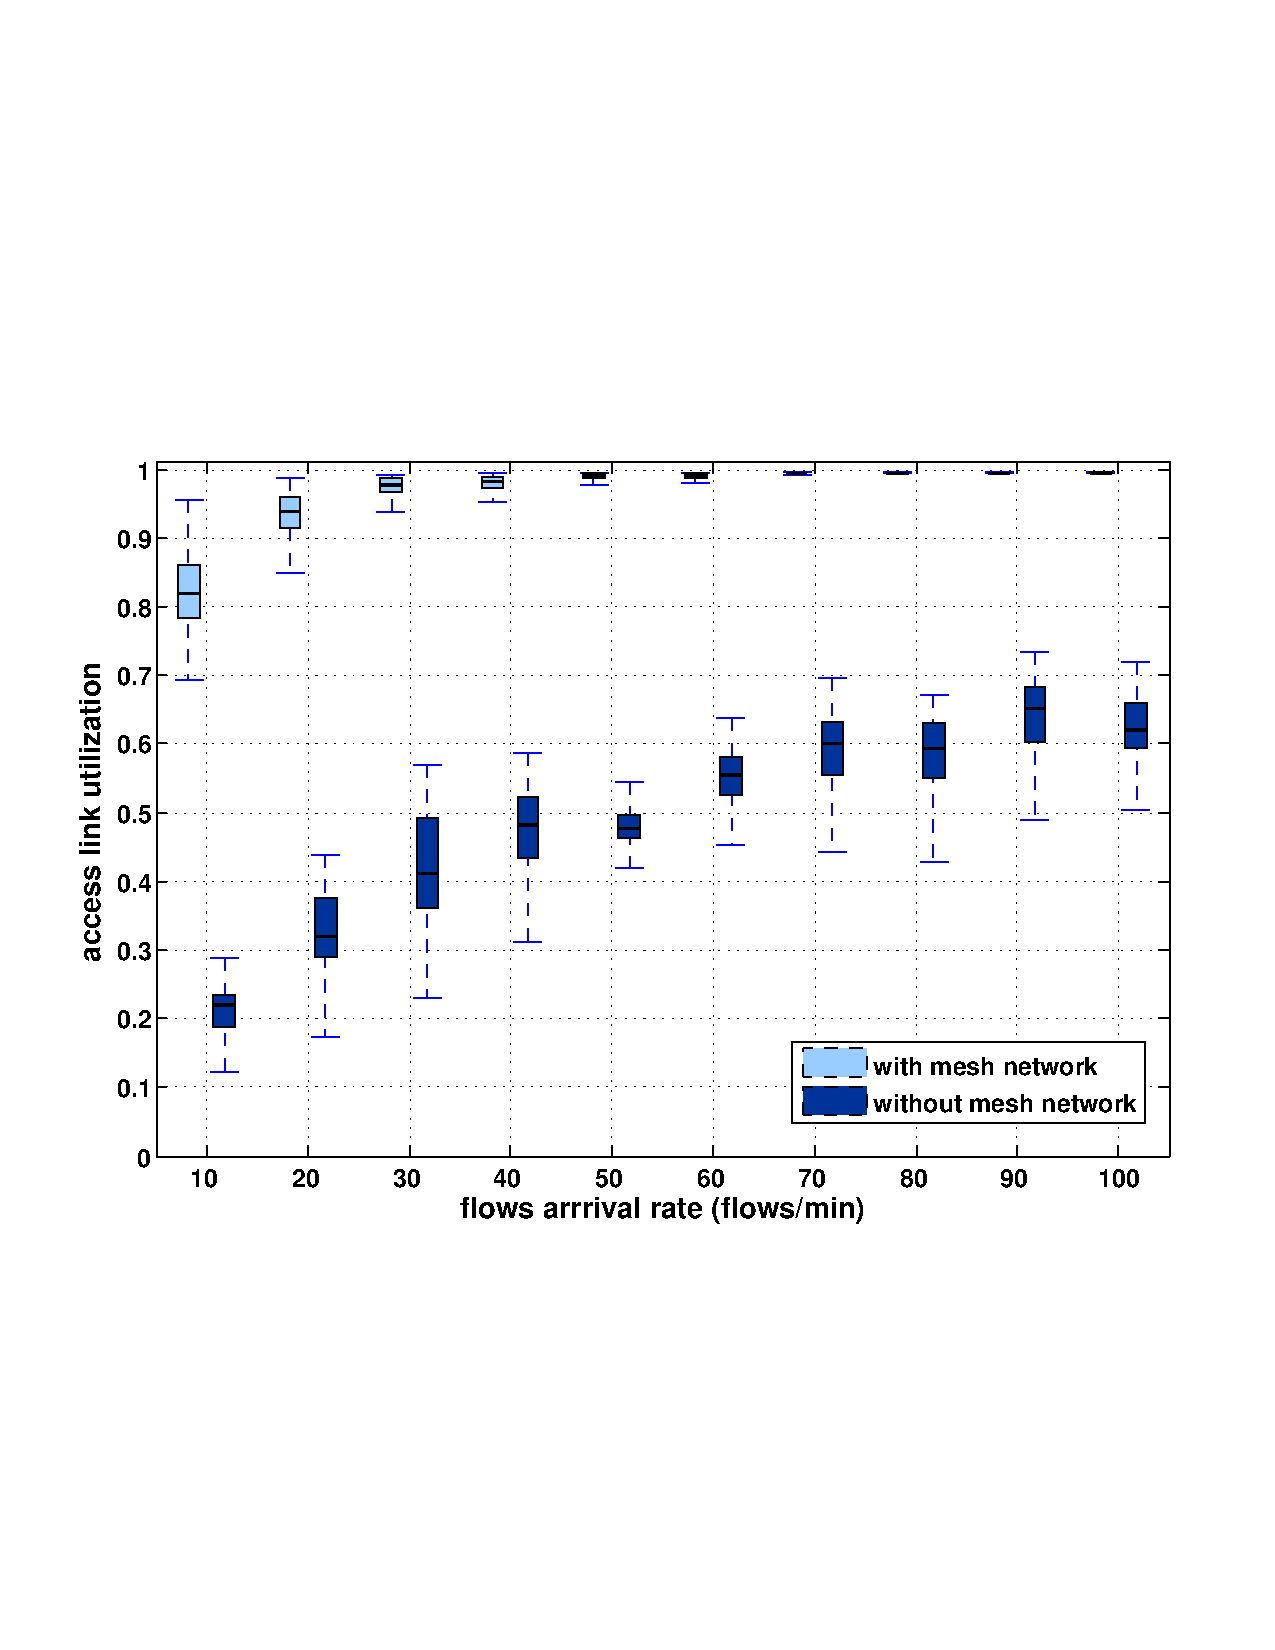
\includegraphics[width=1\linewidth]{../../results/simulation/boxplot2.pdf}  
\caption{Shared bandwidth utilization vs. flow arrival rate.}
\label{fig:utilization_arrival}
\end{center}
\end{figure}


